\documentclass[aps,prstab,showpacs,onecolumn,12pt]{revtex4-1}  
%\documentclass[aps,prstab,showpac,onecolumn,preprint,nofootinbib,12pt]{revtex4-1}  

\usepackage{graphicx}
\usepackage{epsfig}
\usepackage{subfigure}
\usepackage{fancyhdr}
\usepackage{color}
\usepackage{amsfonts}
\usepackage{amsmath}
\usepackage{amssymb}
\usepackage{dcolumn}
\usepackage{bm}
\usepackage{indentfirst}
\usepackage{rotating}
\usepackage{moreverb}

\setlength{\textwidth}{6.5in}
\setlength{\textheight}{8.5in}
\setlength{\topmargin}{0in}
\setlength{\oddsidemargin}{0.0in}
\setlength{\evensidemargin}{0.0in}
\setlength{\rightmargin}{0.0in}

\makeatletter

\begin{document}

\title{Tracking Simulation of Third-Integer Resonant Extraction \\ for Fermilab's Mu2e Experiment}
\author{Chong Shik Park}
\affiliation{Fermi National Accelerator Laboratory, PO Box 500, Batavia, IL 60510}
\date{\today}

\begin{abstract}
The Mu2e experiment at Fermilab requires acceleration and transport of intense proton beams in order to deliver stable, uniform particle spills to the production target. To meet the experimental requirement, particles will be extracted slowly from the Delivery Ring to the external beamline. Using Synergia2, we have performed multi-particle tracking simulations of third-integer resonant extraction in the Delivery Ring, including space charge effects, physical beamline elements, and apertures. A piecewise linear ramp profile of tune quadrupoles was used to maintain a constant averaged spill rate throughout extraction. To study and minimize beam losses, we implemented and introduced a number of features, beamline element apertures, and septum plane alignments. The RF Knockout (RFKO) technique, which excites particles transversely, is employed for spill regulation. Combined with a feedback system, it assists in fine-tuning spill uniformity. Simulation studies were carried out to optimize the RFKO feedback scheme, which will be helpful in designing the final spill regulation system.
\end{abstract}

\pacs{29.27.-a, 41.85.-p}
\maketitle

\setcounter{tocdepth}{10}

%\tableofcontents

%%%%%%%%%%%%%%%%%%%%%%%%%%%%%%%%%%%%%%%%%%%%%%%%%%
\section{\label{sec:intro}Introduction}

The goal of the Mu2e project at Fermilab is to search for charged lepton flavor violating processes of a muon converting to an electron by measuring the branching ratio for coherent neutrino-less conversion in the field of a nucleus~\cite{mu2e0, mu2e1}. The experiment requires slow resonant extraction from Fermilab's Delivery Ring. A batch of protons from the Booster is transported to the Recycler Ring, where the beam is rebunched into four buckets, which are transferred individually to the Delivery Ring. These high intensity beams will be extracted one at a time from the Delivery Ring using slow resonant extraction and delivered to the production target through the external beamline. This paper describes multi-particle tracking simulations of third-integer resonant extraction in the Delivery Ring for the Mu2e experiment. 

The third-integer resonance was first considered and studied because the Delivery Ring has a three-fold symmetry
and its operating tune, $\nu_{x} = 9.765$, was already close to a third-integer resonance, 29/3. 
It was preferred to the half-integer resonance because of lower beam losses at the septum and a higher extraction efficiency.

Two harmonic sextupole circuits in two of the Delivery Ring's straight sections excite the resonance. In order to slowly extract particles, the tune of the ring is gradually adjusted by increasing strengths of three tune-control quadrupoles placed near the middle of each straight section. Two electrostatic septa, one Lambertson magnet, and one C-magnet provide separations and deflections of the extracted beam from the circulating beam. Families of sextupoles are used to adjust and correct machine chromaticity. To finely control the spill rate, an RF Knock-Out (RFKO) feedback system is introduced consisting of an RF kicker, spill monitor, and feedback control unit. Table~\ref{table:param} gives machine and beam parameters of the Delivery Ring for the Mu2e resonant extraction.

\begin{table*}[!bp]
    \begin{tabular}{rrr}
    \hline
     Parameters                & Value              & Units         \\
    \hline
      Beam Momentum     & 8.886    & GeV/c   \\
      Beam Intensity/Spill         &  1 & Tp ($10^{12}$ protons)       \\
      $B \rho$                  & 29.650             & T-m           \\
      Bunch Length (rms)        & 40                 & nsec          \\ 
      95 \% invariant normalized emittance & 20     & $\pi$ mm-mrad \\
      Ring Circumference  & 505.283            & m             \\
      Resonant Tune($\nu_{x})$   & 29/3 &  \\
      Bare Tunes, ($\nu_{x0}$, $\nu_{y0}$)   & (9.65, 9.78)   &    \\
      Spill Duration &  54  & msec \\
      $N_{\text{turn}} / {\text{spill}}$    & 31,795   &    \\
      Protons per pulse     & 31.5  &  Mp ($10^{6}$ protons)  \\
      Harmonic Number           & 4                  &               \\
      RF Frequency              & 2.36               & MHz           \\
      RF Peak Voltage                & 10                 & kV            \\
    \hline
    \end{tabular}
    \caption{\label{table:param}Beam and Machine Parameters}
\end{table*}

We studied the beam dynamics of third-integer resonance extraction in this context using the multi-particle simulation package Synergia2, which already has been used for simulations of other accelerators~\cite{synergia2}. It is capable of tracking millions or billions of macro-particles in single-bunch or multi-bunch modes with various collective effects (esp., space charge and wake fields) and apertures (e.g., circular, elliptical, polygon, etc.). A beam optics code, CHEF, provides single-particle dynamics, including linear and nonlinear optics, direct symplectic tracking through beamline elements, arbitrary order polynomial transfer maps, and other physical and computational features~\cite{chef}. Using Synergia2, we successfully carried out multi-particle tracking simulations for third-integer resonant extraction including space charge effects as well as physical beamline elements and apertures.

There were two main efforts required to realize simulation of third-integer resonant extraction with Synergia2. The first was handling lattice elements in the ring to extract particles using the third-integer resonance model; the second was manipulating the machine parameters in order to make the beam meet the experimental requirement. With numerical optimization studies, a stable spill structure could be achieved by a piecewise linear ramp profile of the tune-quadrupole circuit. A preliminary simulation study showed that using the RFKO feedback system can yield better spill uniformity when power supply ripples are present. Synergia2 is now ready to fully simulate resonant extraction for the Mu2e experiment and to study the spill regulation schemes. More numerical studies and challenges are required to find optimal working points in the machine and to optimize beam manipulations for the experiment.

This paper is outlined as follows. Sec.~\ref{sec:spacecharge} presents space charge effects with Synergia2 during the extraction process. Sec.~\ref{sec:resonance} describes the third-integer resonance model with harmonic sextupole circuits. In Sec.~\ref{sec:tune}, we discuss how to control spills with the tune-control circuits and how to achieve averaged uniform spills with the piecewise linear ramp profile. Extraction beamline elements and beam loss measurements are addressed in Secs.~\ref{sec:septum} and~\ref{sec:aperture}, respectively. Sec.~\ref{sec:rfko} describes regulating the spill rate with the RFKO feedback system.

%%%%%%%%%%%%%%%%%%%%%%%%%%%%%%%%%%%%%%%%%%%%%%%%%%
\section{\label{sec:spacecharge}Space Charge Effects}

The Mu2e experiment requires high intensity beams, $10^{12}$ protons per bunch, so space charge effects will be important during extraction. Self-defocusing space charge fields induce betatron tune shifts within the core of the beam, eventually affecting the spill rate and beam losses~\cite{pac11}.

\begin{figure*}[!btp]
  \subfigure[Beam Intensities]{
    \includegraphics[width=.45\textwidth]{img/fig1a.png}
    \label{fig:fig1a}}
  \subfigure[Tune Footprint]{
    \includegraphics[width=.45\textwidth]{img/fig1b.png}
    \label{fig:fig1b}}
  \caption{\label{fig:fig1}(Color) (a) Intensities of circulating beam during a spill with and without space charge effects. (b) Tune footprint measured at turn 1000. Resonance lines are drawn up to the 6th order: (color: 4th-orange, 5th-green, and 6th-blue).}
\end{figure*}

Synergia2 has several space charge solvers including those with 2.5D and 3D open boundary conditions. For the Mu2e extraction simulation, 2.5D and 3D open Hockney algorithms~\cite{hockney} were mainly used on \mbox{$64\times 64 \times 128$} grid cells with 240 space charge kicks per turn. Benchmark studies have shown that the 2.5D open Hockney solver is sufficient and saves a substantial amount of computational time compared to the 3D solver. To confine the bunch longitudinally, an RF cavity was located in one of the straight section and operated with harmonic number $h=4$, at frequency \mbox{$f_{RF} = 2.36$ MHz}, and voltage \mbox{$V_{RF} = 10$ kV}. With a 40~ns RMS bunch length and a \mbox{20 $\pi$ mm-mrad} normalized initial emittance, \mbox{$\Delta p / p \approx 0.002$}.

For a uniform spill of particles, as required by the experiment, the intensity of the circulating beam should be decreasing at a constant rate.
%Using the same ramp profile of tune-quad strengths during the extraction (more details of the ramp profile will be discussed in Sec.~\ref{sec:tune}), 
Fig.~\ref{fig:fig1a} shows comparisons of circulating beam intensities with and without space charge effects as a spill progresses.
After the piecewise linear tune ramp has been optimized, the intensity curve produced by the 2.5D space charge solver lies on top
of the ideal so that they are indistinguishable at the scale of the figure.
Turning off space charge makes it clear that it produces an operational effect that cannot be ignored.
% It is clear that beam intensities are decreasing in different rates with/without space charge effects.
Moreover, space charge induced tune shifts depend on the betatron amplitude of particles, the core of the beam having a larger tune shift than the beam halo. The overall effect of self-defocusing fields reduces the betatron tune of particles downward from the bare tune. In Fig.~\ref{fig:fig1b}, a tune distribution at a working point of $(\nu_{x}, \nu_{y}) \simeq (9.65, 9.78)$ shows the downward spread of particles' tunes.

%%%%%%%%%%%%%%%%%%%%%%%%%%%%%%%%%%%%%%%%%%%%%%%%%%
\section{\label{sec:resonance}Third-Integer Resonance with Harmonic Sextupole Circuits}

In the Delivery Ring for the Mu2e experiment, two orthogonal groups of three sextupoles each located in two of straight sections form the harmonic sextupole circuits. In strong sextupole fields, the stable motion of the particles is limited by the certain area in the phase space, called the separatrix, when the horizontal tune is close to a resonance value, $n/3$.
Based on perturbation theory, the Hamiltonian of the third-integer resonance model can be written as
\begin{equation}
  H = \Delta \nu I - ( g e^{-i 3 \phi} + g^{*} e^{i 3 \phi} ) I^{3/2} + ... .
  \label{eqn:eqn1}
\end{equation}
where $\Delta \nu = \nu_{x} - 29/3$ is the difference between the horizontal and resonant tunes, $(\phi,I)$ are linear angle-action coordinates, and $g$ is the resonance coupling constant. The resonance coupling constant, $g$, is linear functional of the harmonic sextupole strength and phase distribution, defined as 
\begin{equation}
  g  = \frac{i}{6 \sqrt{2}} \frac{1}{4 \pi}
          \sum_{\text{sextupoles}} \frac{B^{\prime\prime} l}{B \rho}
          \beta^{3/2}_{x} e^{- i 3 \left( \psi_{x} 
                                           - \Delta \nu \cdot \theta \right) },
\label{eqn:eqn2}
\end{equation}
where $\beta_{x}$, $\psi_{x}$, and $\theta$ are lattice functions measured at each harmonic sextupole location. 
A detailed derivation is given in reference~\cite{Leo}. 

The strengths of the harmonic sextupoles are determined by the initial tune of the ring and the emittance of the injected beam,
\begin{equation}
  |g| = \frac{ | \Delta \nu | }{ \sqrt { 2 \sqrt{3} \epsilon_{x} } } ,
  \label{eqn:eqn3}
\end{equation}
where $\epsilon_{x}$ is the horizontal emittance of the central stable region. Eq.~(\ref{eqn:eqn3}) is used to set initial sextupole strengths to enclose all particles inside of the separatrix after injection. The phase of the coupling constant, given by Eq.~(\ref{eqn:eqn2}), determines the orientation of the separatrix. In the Delivery Ring, the contributions from the two harmonic sextupole circuits are almost orthogonal, enabling control of $g$'s amplitude and phase with two ``knobs''~\cite{Leo}.

\begin{figure} [!tbp]
  \includegraphics[width=3in]{img/fig2.png}
  \caption{\label{fig:fig2}(Color) Particle distribution and the third-integer resonance near the beginning of extraction plotted using normalized coordinates. Stable particles are within the central region. Particles on the outgoing branches are being extracted.}
\end{figure}

When a beam is injected in the simulation, the harmonic sextupole fields are gradually ramped from zero to the desired strengths for the third-integer resonance in the first 100 turns. They are then held constant at their final settings during extraction, while the tune is moved toward resonance. Fig.~\ref{fig:fig2} shows a particle distribution in normalized coordinates with the third-integer separatrix superposed for \mbox{$\nu_{x0} = 9.65.$} The phase of the resonance coupling constant is adjusted so that the orientation of the separatrix is parallel to the horizontal line in the normalized coordinates. 

%%%%%%%%%%%%%%%%%%%%%%%%%%%%%%%%%%%%%%%%%%%%%%%%%%

\section{\label{sec:tune}Slow Extraction with Tune-Control Circuits}

After the third-integer resonance is excited, particles are extracted by shrinking the separatrix, in principle either by moving the tune into resonance or by increasing the harmonic sextupole strengths. However, the latter is impractical since very large sextupole strengths would be needed to extract small amplitude particles, and non-linearities dominate. Instead, extraction is achieved by driving $\Delta \nu$ to zero.

Controlling the machine's tune requires initially placing the horizontal tune slightly below \mbox{$\nu_{x} = 29/3$} and then carefully moving it into the resonance by increasing strengths in the tune-quadrupole circuit. The initial machine tune is set by normal bussed quadrupoles in the Delivery Ring. Trim quadrupoles will be installed near the center of each of the ring's three straight sections. They will be ramped to adjust the tune during extraction, with strengths given by Eq.~(\ref{eqn:eqn4}).
\begin{equation}
  \Delta \nu - \Delta \nu_{0} = \frac{1}{4 \pi} \sum_{\text{tune-quads}} \beta_{x} \frac{B^{\prime} l}{(B \rho)}
  \label{eqn:eqn4}
\end{equation}

Since the experiment requires the delivery of uniform particle flows to the production target, the spill rate should remain constant during extraction; intensity of the circulating beam should decrease linearly.
Extraction simulations predict that spills will not be uniform with a linear ramp of tune-quad strengths. As seen in Fig.~\ref{fig:fig3}, circulating beam intensity does not decrease at a constant rate; the ideal intensity profile, corresponding to a uniform spill, is the straight line drawn in orange.

\begin{figure} [!tbp]
  \includegraphics[width=3in]{img/fig3.png}
  \caption{\label{fig:fig3}(Color) When tune-quads are linearly ramped, the beam intensity is not linearly decreasing.}
\end{figure}

\begin{figure*} [!tbp]
  \subfigure[Tune-quad strength and machine tune]{
    \includegraphics[width=.45\textwidth]{img/fig4a.png}
    \label{fig:fig4a}}
  \subfigure[Beam intensity]{
    \includegraphics[width=.45\textwidth]{img/fig4b.png}
    \label{fig:fig4b}}
  \caption{\label{fig:fig4}(Color) (a) Tune-quad strength, and machine tune with the piecewise linear ramp profile for the first 1000 turns, and (b) corresponding beam intensity. Each interval has the same color code.}
\end{figure*}

We introduce a piecewise linear ramp profile to control the tune-quad circuit via a feed-forward loop. 
The whole extraction period is partitioned into small intervals, with tune-quad strengths varying linearly within each interval.  These variations satisfy initial and final tune-quad settings as well as continuity of the ramp. The initial tune-quadrupole strengths are set to zero, and their final values can be calculated from Eq.~(\ref{eqn:eqn4}) by setting $\Delta \nu$ to zero. For a given interval, tune-quad strengths are numerically determined to make the spill as uniform as possible.

Fig.~\ref{fig:fig4a} shows ramp profiles of tune-quad strengths and machine tune for the first 1000 turns, while Fig.~\ref{fig:fig4b} is the corresponding (circulating) beam intensity. By changing the slope of the ramp profile at every 200 turns, the beam intensity remains close to the ideal.
A Gaussian distribution was used to populate the phase space of the injected beam.
As the separatrix forms, outlier particles in its vicinity or outside the central region stream outward even before the tune-quad ramp begins.
This accounts for the sudden drop in beam intensity near the beginning.

\begin{figure*} [!tbp]
  \subfigure[Beam intensity]{
    \includegraphics[width=.45\textwidth]{img/fig5a.png}
    \label{fig:fig5a}}
  \subfigure[Spill rate]{
    \includegraphics[width=.45\textwidth]{img/fig5b.png}
    \label{fig:fig5b}}
  \caption{\label{fig:fig5}(Color) With the piecewise linear ramp profile, the spill structure is uniform within $\pm20 \; \%$ tolerance, while the beam intensity is decreasing linearly.}
\end{figure*}

Fig.~\ref{fig:fig5} shows simulation results of beam intensity and spill rate with an optimal ramp profile. As seen in Fig.~\ref{fig:fig5a}, the beam intensity is decreasing close to the ideal one. Spill structures are varying within \mbox{$\pm 20\%$} while satisfying the required tolerance, \mbox{$\pm 50\%$}, of the experiment. Spill fluctuations are mainly caused by the piecewise ramp of tune-quad strengths. On top of those variations, there is also a statistical noise induced by the number of macro particles. Therefore, spill fluctuations in the simulation could be reduced more by further optimizing the ramp profile as well as by increasing the number of macro-particles.


%%%%%%%%%%%%%%%%%%%%%%%%%%%%%%%%%%%%%%%%%%%%%%%%%%
\section{\label{sec:septum}Septum Design}

During extraction, unstable particles traveling along separatrix branches are separated from the circulating beam and extracted by passing through electrostatic septa and a magnetostatic Lambertson magnet. For the Mu2e experiment, two septa and one Lambertson magnet are placed in the straight section in which harmonic sextupoles are not installed. The Lambertson magnet has 1.5~m length, and its magnetic field strength is about 1~Tesla. In each septum, an electrostatic field of 100 kV will be applied across a 14~mm gap between the foil plane and anode. In the simulations reported here, we used two septa with an equal length of 1.5~m. However, dedicated MARS beamline simulations focusing on the extraction beamline show that asymmetric lengths of two septa will have better extraction efficiency~\cite{mars}.

Synergia2 is capable of propagating particles inside of a septum element with its real geometry. That is, a septum element in the simulation can be specified with its length, voltage, foil's horizontal position and width, and gap size. Within a finite length septum element, circulating particles are propagated in the drift space, while outgoing particles in the field region of the septum are kicked by the electrostatic field. In our simulations, protons streaming outward from the circulating beam are kicked at two septa, propagated to the Lambertson magnet, and then removed. 

Beam losses at septa are a key factor in the septum design process. Due to the finite thickness of a septum foil, a fraction of the particles will hit the foil. Some could cross the septum foil plane, and be either partially kicked by the electrostatic field or scattered by the foil. These would likely be lost within the ring.

\begin{figure*} [!tbp]
  \subfigure[12.5 $mm$]{
    \includegraphics[width=.45\textwidth]{img/fig6a.png}
    \label{fig:fig6a}}
  \subfigure[14.0 $mm$]{
    \includegraphics[width=.45\textwidth]{img/fig6b.png}
    \label{fig:fig6b}}
  \caption{\label{fig:fig6}(Color) $2I_{x}$ (2 $\times$ action coordinates) ($\mu$m) vs. $x$ (horizontal) coordinates (mm) for two different choices of the septum foil position. Particles are moving toward the negative $x$-direction.}
\end{figure*}

The probability of hitting a septum's foil is reduced by increasing the step size,
the displacement of a proton in three turns around the ring. However, machine acceptance places limits on the step size. When particles are streaming away, their transverse motion is bounded by the machine acceptance. If a particle reaches the aperture limit, it will be lost somewhere in the ring before being kicked by the septum field. Fig.~\ref{fig:fig6} shows two distinct versions of a septum's foil position and beam losses. By moving the foil closer to the central orbit, one can avoid the limit of the machine acceptance of the Delivery Ring, 35 $\pi$ mm-mrad. In doing so, one should also consider that the foil is not to interfere the circulating beam, which is less than 8 mm (not shown in Fig.~\ref{fig:fig6}). When a particle (color: blue x) is streaming along the separatrix (color: red cross), its motion is bounded by the machine acceptance (color: cyan line). With a proper septum foil position (12.5 mm, color: black double lines) shown in Fig.~\ref{fig:fig6a}, more particles can avoid the machine acceptance. For 14 mm foil position in Fig.~\ref{fig:fig6b}, however, particles (color: green star) beyond the aperture limit will be lost. In both cases, there are particle losses (color: purple star) due to hitting the septum foil.

\begin{figure*} [!tbp]
  \subfigure[Before Rotation]{
    \includegraphics[width=.45\textwidth]{img/fig7a.png}
    \label{fig:fig7a}}
  \subfigure[After Rotation]{
    \includegraphics[width=.45\textwidth]{img/fig7b.png}
    \label{fig:fig7b}}
  \caption{\label{fig:fig7}(Color) Particles on a separatrix branch are tracked (a) before and (b) after the septum plane rotation. With a proper rotation of the septum plane, kicked particles by the electrostatic field are clearly separated from the circulating beam with less beam loss.}
\end{figure*}

Moreover, the angle of the septum plane with respect to the central orbit is also important in the consideration of beam losses. Because of beam angle spread or septum misalignment, particles may be scattered by the foil plane within the septum. Their number must be minimized, because this leads to losses due to a partial kick and insufficient deflection by the electrostatic field or to foil scattering.

Fig.~\ref{fig:fig7} shows the horizontal coordinates ($x$) of particles sitting on the separatrix branch at the extraction beamline in the vicinity the first septum. Without a rotation of the septum plane (Fig.~\ref{fig:fig7a}), some particles (color:green) cross the septum plane during passage through the septum. With a proper rotation (Fig.~\ref{fig:fig7b}), however, kicked (color:blue) and circulating (color:red) particles are clearly separated after passing the septum element. The plane of the second septum in the Delivery Ring is also rotated in the design and simulation, but its angle has the opposite sign since it is located downstream of a focusing quadrupole, and therefore the particles' directions are positive. 

%%%%%%%%%%%%%%%%%%%%%%%%%%%%%%%%%%%%%%%%%%%%%%%%%%

\section{\label{sec:aperture}Beam Loss Measurements with Apertures}

Besides spill uniformity, it is also important to minimize beam losses more than for the experiment activation limits, etc. Our goal is to lose no more than 2\% of the beam. In order to measure beam losses in accelerators, Synergia2 implemented various apertures, such as circular, elliptical, polygon, and wire-elliptical apertures. By specifying apertures of each beamline element in the ring, one can measure when and where beam losses occur during the simulation. For example, a drift space with a circular or elliptical beam pipe is able to detect out of bound particles with the corresponding aperture.

\begin{figure*}[!tbp]
  \subfigure[polygon aperture with 64 vertices]{
    \includegraphics[width=.45\textwidth]{img/fig8a.png}
    \label{fig:fig8a}}
  \subfigure[Particles filtered by apertures]{
    \includegraphics[width=.39\textwidth]{img/fig8b.png}
    \label{fig:fig8b}}
  \caption{\label{fig:fig8}(Color) (a) The star-shaped beam pipe for quadrupoles are formed with 64 vertices. The pseudo-circular aperture inside of the polygon filter particles. (b) As a test, particles in a largely expanded distribution are filtered by polygon and wire-elliptical apertures.}
\end{figure*}

Quadrupole magnets in the Delivery Ring have star-shaped beam pipes with 4-pole shapes, as seen in Fig.~\ref{fig:fig8a}. Synergia2's polygon aperture utilizes a winding number algorithm to make beam loss measurements for such complex shaped beam pipes. 
Multiple vertices can realize an arbitrary shape, however, this algorithm has a drawback in computational time with a large number of macro-particles, since it has to check all particles with every vertex of the polygon. As shown in Fig.~\ref{fig:fig8a}, we introduced an ``inscribed circle" (color: blue circle), which filters particles before applying arbitrary shape aperture (color: red curve). Winding numbers then need to be calculated only for particles outside the circle, saving significant computational time.

Beam losses at the septa are typically many times larger than the distributed losses in the ring. With the physical geometry of a septum, we need to detect the following losses: (1) particles hitting the septum foil at the entrance, (2) particles crossing the septum plane inside of it, and (3) particles hitting the anode and beam pipe. The wire-elliptical aperture is designed to measure these. Fig.~\ref{fig:fig8b} shows an example of lost particles when a largely expanded beam passes polygon and wire-elliptical apertures.
Particles outside of the polygon shape are filtered by the polygon aperture, which is the main aperture for quadrupoles. Particles inside of the ellipse sifted with the wire-elliptical aperture by hitting wire or anode of the septum. 

The septum geometry (position and angle) and sextupole field are chosen to maximize step size and to minimize beam losses within the limits of machine acceptance (see Sec.~\ref{sec:septum}). Whereas the apertures of elements in the ring are described and checked in the model, they can be used to determine critical locations, however, they do not fully reflect the real machine acceptance. Because it is important to introduce the real acceptance into our model, it has been enforced by adding an artificial ``phase-space aperture'' of 35~$\pi$~mm-mrad, which is placed just upstream of the electrostatic septum. While physical apertures limit a particle's spatial coordinates, the phase-space aperture restrains both spatial and momentum coordinates, e.g., $(x, x^{\prime})$ or $(y, y^{\prime})$. Therefore, particles are constrained by an elliptical aperture in phase space with boundary at the maximum action consistent with the machine aperture; for example,
\begin{equation}
  I_{x}^{\text{max}} = \frac{x^{2} +  ( \alpha_{x} x + \beta_{x} x^{\prime} )^{2}}{2 \beta_{x}},
  \label{eqn:eqn6}
\end{equation}
where $\alpha_{x}$ and $\beta_{x}$ are the local horizontal lattice functions.

%%%%%%%%%%%%%%%%%%%%%%%%%%%%%%%%%%%%%%%%%%%%%%%%%%
\section{\label{sec:rfko}Spill Control with RFKO Feedback System}

Sec.~\ref{sec:tune} shows that a reasonably uniform spill structure was achieved in Synergia2 tracking simulations with a piecewise linear ramp of tune-quad strengths. However, fast variations of spills still could be substantial because of ``dirt effects,'' such as magnet imperfections or magnet power supply ripples. We have adopted an RF Knockout (RFKO) method to finely control the spill uniformity~\cite{HB10}. A transverse RF system creates an RF field with a narrow bandwidth around the betatron frequency which ``heats'' the beam horizontally and pushes it out of the central stable region of the separatrix.

The RFKO feedback system, comprising the RFKO kicker, spill monitor, and feedback control unit, will be used to minimize spill fluctuations and to regulate spill uniformity. A wall current monitor will be installed in the external beam line and operate as the spill monitor. It will detect signals of beam extracted from the Delivery Ring and send them to the feedback system, which will then calculate strengths of the feedback amplitude, integrated over 100 turns, or so, and apply it to the RFKO kicker~\cite{wcm}.

In order to effectively excite the beam, the RFKO kicker frequency must match the particles' betatron frequency. Since there is a significant tune spread in the beam, a narrow band frequency can match only to a small fraction of the particles. To cover the tune range of all particles, the RF frequency must be frequency-modulated within a bandwidth comparable to the tune spread. A previous study showed that the space charge tune shift alone does not lead to sufficient mixing of coherent oscillations and emittance growth~\cite{HB10}.  For the extraction simulation, we set the chromaticity \mbox{$C_{x} = 1.0$} using chromaticity correction sextupoles. The bandwidth is then determined from the chromatic tune spread, given the momentum spread of the beam. As the machine tune is ramped during the spill, the central frequency of the RFKO kicker must change accordingly.

In this study, we used a linear chirp FM signal for the RF field. The central frequency is matched to the betatron frequency, and the bandwidth covers the betatron tune spread. When the frequency-sweep interval is changed at every 100 turns, its frequency spectrum shows a series of narrow lines around the central frequency. To overcome this feature, we add random phases for each sweep to smear the spectrum. 

In order to test the feedback system, we added artificial power supply ripples to the simulation. Strengths of quadrupoles varied in time with a frequency of 60 Hz and peak-to-peak variations of \mbox{$\pm0.5$ \%} of the designed values. These power supply ripples create large fluctuations in the spill structure. The frequency of the resulting spill rate follows harmonics of the ripple frequency. 

\begin{figure}[!tbp]
  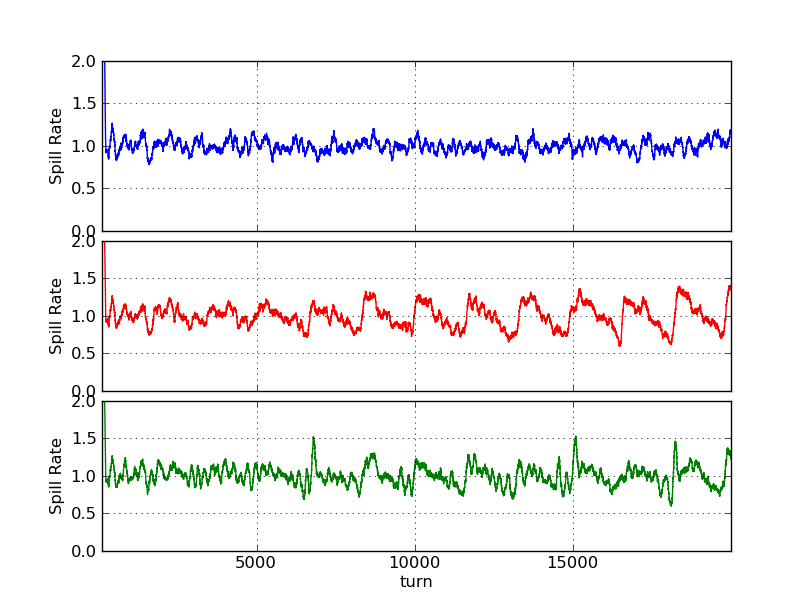
\includegraphics[width=.45\textwidth]{img/fig9.png}
  \caption{\label{fig:fig9}(Color) Normalized spill rates in the presence of power supply ripples: (top) ripples off and feedback off, (middle) ripples on and feedback off, and (bottom) ripples on and feedback on. Power supply ripples bring large fluctuations on the spill rate, and it is improved by the feedback system.}
\end{figure}

To control this behavior, we tried various feedback mechanisms based on the classic PID (Proportional-Integral-Derivative) feedback theory~\cite{pid}.
When we applied only the proportional gain feedback signal, we observed that there were very large oscillations in spill rates. 
One reason for this was latency between the spill monitor and beam responses to RFKO excitations. This results in over-regulations of spill ripples.
Our current best method is to combine dynamical changes of the proportional gain in time with a constant derivative gain.

Fig.~\ref{fig:fig9} shows a comparison of spill rates with and without the feedback loop in the presence of power supply ripples. Power supply ripples drive the oscillations in the spill rate. We observe that fluctuations are improved with the feedback routine, although there remain a few large spikes, as seen at the bottom of Fig.~\ref{fig:fig9}. We expect this performance could be improved further by adding integral gain to the RFKO feedback system. 

\section{\label{sec:conclusion}Conclusion}

Fermilab's Mu2e project requires slow extraction from the Delivery Ring. Using Synergia2, we have successfully demonstrated simulations of third-integer resonant extraction with space charge effects. A stable, uniform spill structure is realized using a piecewise linear ramp profile of the tune-quad circuit. We have implemented septa and a Lambertson magnet with real, physical geometries; their parameters were optimized to enhance the extraction efficiency and to minimize beam losses during the extraction. Various apertures - circular, elliptical, wire-elliptical, and a phase-space aperture to model machine acceptance - were introduced to estimate beam losses around the ring. Feedback simulations show that the RFKO technique could improve the spill structure when magnet power supply ripples are presented. More simulation efforts will be needed to continue optimizing parameters to meet the experiment's requirements. To this end, we have carried out an implementation study of non-linear optimization libraries for Synergia2.

\section{\label{thanks}Acknowledgments}

The author of this paper would like to thank to Drs. James Amundson, Leo Michelotti, and Vladimir Nagaslaev of Fermilab for their great supports and helpful comments in this work. This work was supported by the United States Department of Energy under contract DE-AC02-07CH11359 and the ComPASS project funded through the Scientific Discovery through Advanced Computing program in the DOE Office of High Energy Physics.

\begin{thebibliography}{77}

 \bibitem{mu2e0}
  Mu2e Proposal, Mu2e Document 388-v1, 
  at http://mu2e-docdb.fnal.gov.

  \bibitem{mu2e1}
  Mu2e Accelerator CDR Chapter, Mu2e Document 1324-v11
  at http://mu2e-docdb.fnal.gov.

  \bibitem{synergia2}
  J. Amundson, P. Spentzouris, J. Qiang, and R. Ryne, ``Synergia: An 
  Accelerator Modeling Tool with 3-D Space Charge," J. Comp. Phys. 211 229-248; J. Amundson, ''Synergia2.1: A Framework for Accelerator Simulations,'' in https://cdcvs.fnal.gov/redmine/projects/synergia2.
  
  \bibitem{chef}
  L. Michelotti and J.-F. Ostiguy, ``CHEF: an Interactive Program for Accelerator Optics,'' in PAC'05 Proceedings.
  
  \bibitem{Leo}
  L. Michelotti and J. Johnstone, ``Preliminaries Toward Studying Resonant
  Extraction from the Debuncher," Technical Report, Fermilab, 2009.
  FERMILAB-FN-0842-APC-CD.

  \bibitem{pac11}
  C.S. Park, J. Amundson, J. Johnstone, V.P. Nagaslaev, S. Werkema, 
  ``Space Charge Effect of the High Intensity Proton Beam During the Resonance Extraction for the Mu2e Experiment at Fermilab,'' in PAC'11 proceedings.

  \bibitem{hockney}
  R.W. Hockney and J.W. Eastwood, ``Computer Simulation Using Particles,'' Institute of Physics Publishing, Bristol, 1992.

  \bibitem{mars}
  N. Mokhov, ``MARS15 overview,'' Fermilab-CONF-10/518-APC, 2010; V. Nagaslaev and I. Rakhno, ``MARS Simulations for the Mu2e Delivery Ring Extraction Channel,'' Mu2e Document 3697-v1 at http://mu2e-docdb.fnal.gov.  
  
  \bibitem{HB10}
  V. Nagaslaev, J.F. Amundson, J.A. Johnstone, L. Michelotti, C.S. Park, 
  M.J Syphers, and S.J. Werkema, ``Third Integer Resonance Slow Extraction 
  Scheme for a mu $ \rightarrow $ e Experiment at Fermilab," in HB 2010.

  \bibitem{wcm}
  P. Prieto, ``Wall Current Monitor for fast Spill Measurement,'' Mu2e Document 3627-v4, at http://mu2e-docdb.fnal.gov; P. Prieto, ``RFKO regulation for the Mu2e Resonant Extraction,'' Mu2e Document 3625-v1, at http://mu2e-docdb.fnal.gov.

  \bibitem{pid}
  T. Himel, ``Feedback: Theory and Accelerator Applications,'' Slac-pub-7398, 1997.

\end{thebibliography}

\end{document}
